% This is auto-generated file: do not edit!
% Exported from microMathematics Plus, version 2.15.4


Данный пример демонстрирует
построение и возможности настройки
графиков функций. Построим графики
трёх следующих функций:
\begin{center}\begin{tabular}{c}
  $f(x) := 25 + 10 \cdot sin \left( \sqrt{ \left| x \right| } \right) $
\end{tabular}\end{center}
\begin{center}\begin{tabular}{c}
  $g(x) := \frac{2}{{e}^{ \left| x \right|  / 15}} \cdot f \left( x \cdot 50\right) $
\end{tabular}\end{center}
\begin{center}\begin{tabular}{c}
  $h(x) := min \left( f \left( x\right) ,\, g \left( x\right) \right) $
\end{tabular}\end{center}

Значение аргумента функции, которое
откладывается по оси x, будет
изменяться в интервале от x1 до x2
и содержать N точек:
\begin{center}\begin{tabular}{ccc}
  $N := 300$ &
  $x1 := -30$ &
  $x2 := 30$ \cr
\end{tabular}\end{center}
\begin{center}\begin{tabular}{c}
  $x := \left[ x1,\, x1 + \left( x2 - x1 \right) / N \,..\, x2 \right]$
\end{tabular}\end{center}

После того, как функции и их
аргументы определены, можно
добавить поле графика, используя
кнопку ''Вставить'' на верхней
панели инструментов или кнопку
''Вставить график функции'' на
нижней панели:
\begin{center}\begin{tabular}{c} 
\includegraphics[resolution=320]{graphics/function_plot_fig1.png} \end{tabular}\end{center}
\begin{center}\begin{tabular}{c} 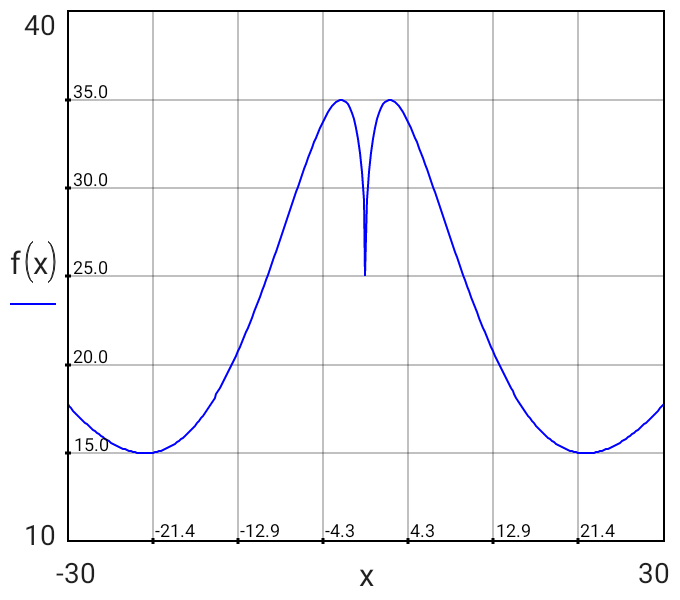
\includegraphics[resolution=320]{graphics/function_plot_fig2.png} \end{tabular}\end{center}

Функция, для которой строится
график, задаётся в левом среднем
поле. В нём можно использовать
любые встроенные или введённые
ранее функции, а также выражение,
содержащее любые операции.

В нижнем среднем поле указывается
аргумент функции, для которого
строится график. Аргументом может
быть как переменная интервального
типа, так и любое выражение, явно
содержащее такую переменную.

Остальные четыре поля служат для
задания областей значений
аргумента и функции. Если эти поля
оставить пустыми, то программа
вычислит их автоматически. Однако,
эти автоматические значения можно
редактировать и изменять вручную.

Можно строить в одном поле графики
сразу нескольких функций. Для
добавления ещё одной функции
необходимо выделить (долгим
нажатием в левом среднем поле) ту
функцию, после которой нужно
добавить новую, и затем нажать
кнопку ''Вставить аргумент'' на
нижней панели инструментов:
\begin{center}\begin{tabular}{c} 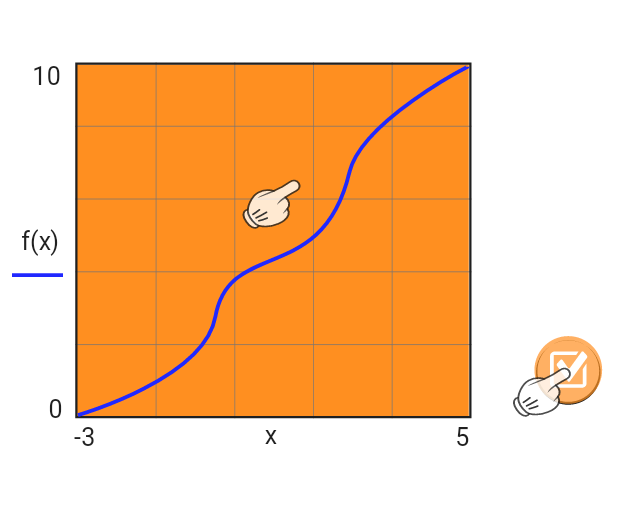
\includegraphics[resolution=320]{graphics/function_plot_fig3.png} \end{tabular}\end{center}
\begin{center}\begin{tabular}{c} 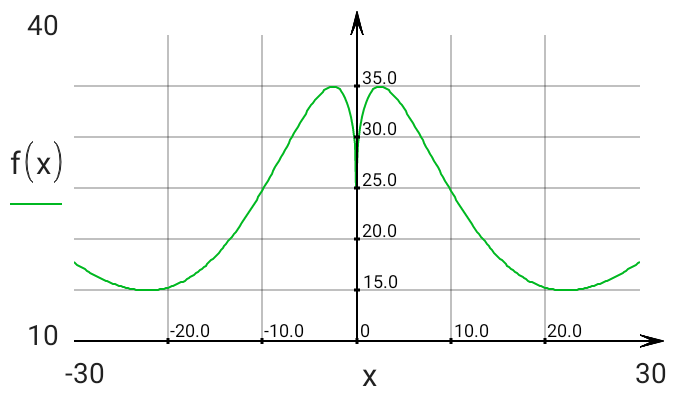
\includegraphics[resolution=320]{graphics/function_plot_fig4.png} \end{tabular}\end{center}

При долгом нажатии по центру
графика появятся контекстное меню
и плавающая кнопка ''Настройки
объекта''.
\begin{center}\begin{tabular}{c} 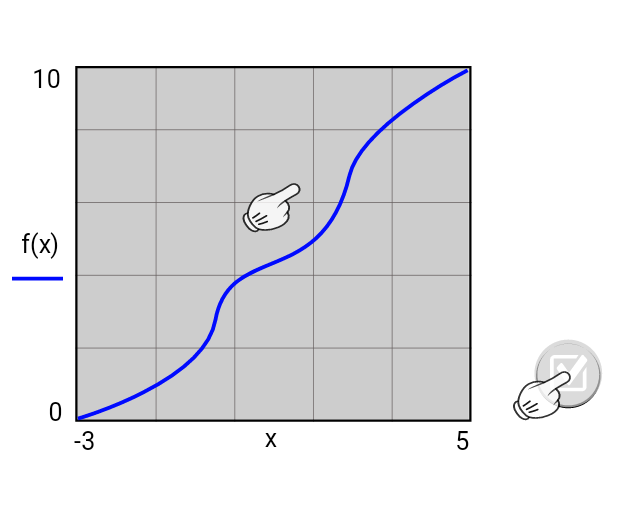
\includegraphics[resolution=320]{graphics/function_plot_fig5.png} \end{tabular}\end{center}

При нажатии на эту кнопку откроется
окно настроек графика, где можно
изменить как размер, так и стиль
области графика. К примеру, мы
можем уменьшить высоту и включить
координатные оси вместо рамки:
\begin{center}\begin{tabular}{c} 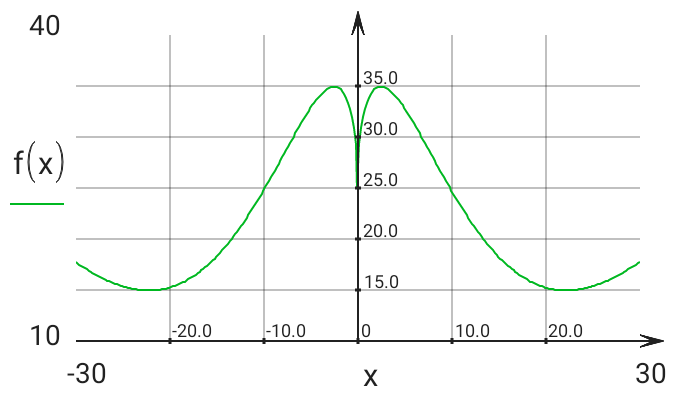
\includegraphics[resolution=320]{graphics/function_plot_fig6.png} \end{tabular}\end{center}

Толщину, цвет и стиль линий графика
можно изменить в окне ''Настройка
линии''. Это окно вызывается долгим
нажатием на линию-маркер,
расположенную под выражением
функции слева от поля графика:
\begin{center}\begin{tabular}{c} 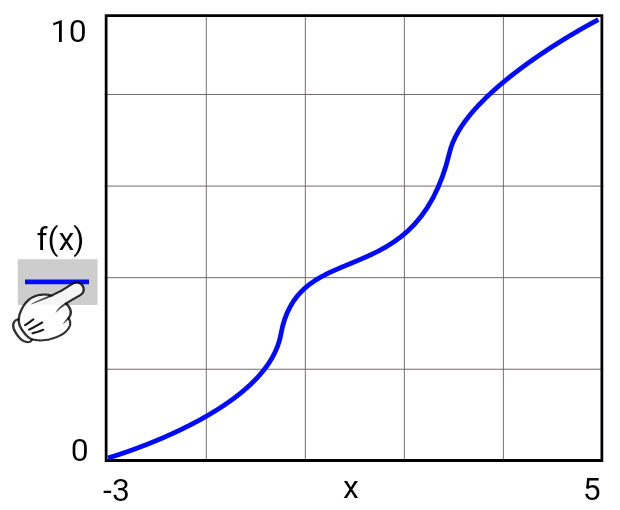
\includegraphics[resolution=320]{graphics/function_plot_fig7.png} \end{tabular}\end{center}

Например, построим пунктирный
график:
\begin{center}\begin{tabular}{c} 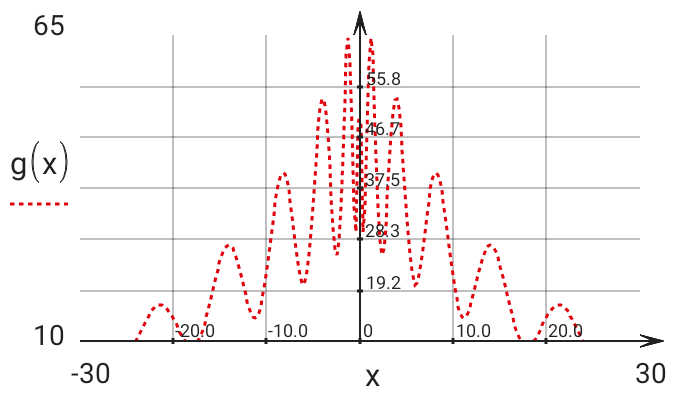
\includegraphics[resolution=320]{graphics/function_plot_fig8.png} \end{tabular}\end{center}

Количество линий сетки по
горизонтали и вертикали, а также
цвет линий сетки можно изменить в
окне ''Настройка сетки''. Это окно
вызывается долгим нажатием в
пустые области снизу от графика,
между минимальным значением и
выражением для аргумента, а также
между аргументом и его
максимальным значением:
\begin{center}\begin{tabular}{c} 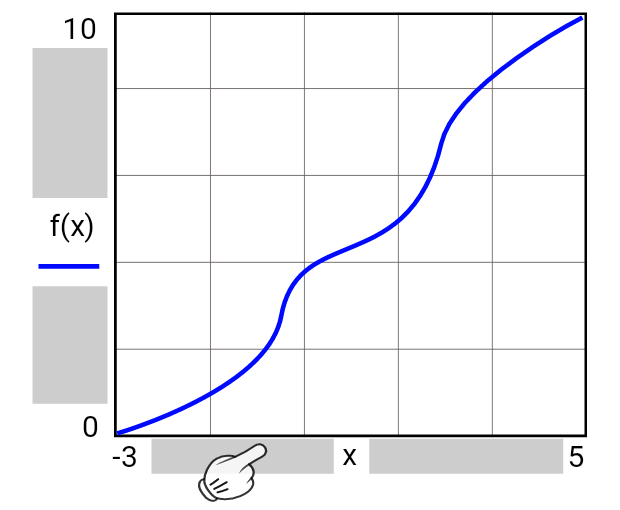
\includegraphics[resolution=320]{graphics/function_plot_fig9.png} \end{tabular}\end{center}
\begin{center}\begin{tabular}{c} 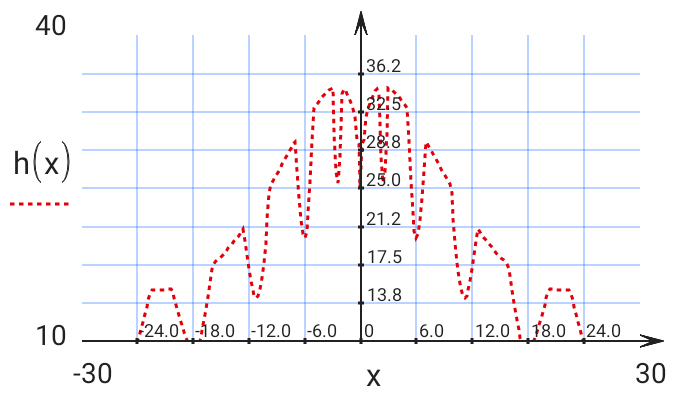
\includegraphics[resolution=320]{graphics/function_plot_fig10.png} \end{tabular}\end{center}

Чтобы полностью отключить сетку,
необходимо задать нулевое
количество линий по горизонтали и
вертикали.